\documentclass[tikz,border=8pt]{standalone}
% Shared look for every TikZ diagram. Load with \input{../../tools/tikz-style.tex}
\usepackage[T1]{fontenc}
\usepackage{lmodern}
\renewcommand{\sfdefault}{lmr}  % diagrams use the same serif as the text
\usetikzlibrary{arrows.meta, positioning, shapes.geometric, calc, fit, backgrounds}
\definecolor{cblue}{HTML}{4C78A8}
\definecolor{corange}{HTML}{F58518}
\definecolor{cgreen}{HTML}{54A24B}
\definecolor{cred}{HTML}{E45756}
\definecolor{cpurple}{HTML}{B279A2}
\definecolor{cgrey}{HTML}{6B6B6B}
\tikzset{
  every picture/.style={font=\sffamily, line width=1.2pt},
  box/.style={draw=#1, fill=#1!12, rounded corners=4pt, align=center, inner sep=7pt, minimum height=1.1cm},
  box/.default=cgrey,
  arrow/.style={-{Stealth[length=3mm]}, draw=cgrey, line width=1.4pt},
  title/.style={font=\sffamily\bfseries\Large},
  note/.style={font=\sffamily\small, text=cgrey, align=center},
}
\AtBeginDocument{\hyphenpenalty=10000 \exhyphenpenalty=10000}

\begin{document}
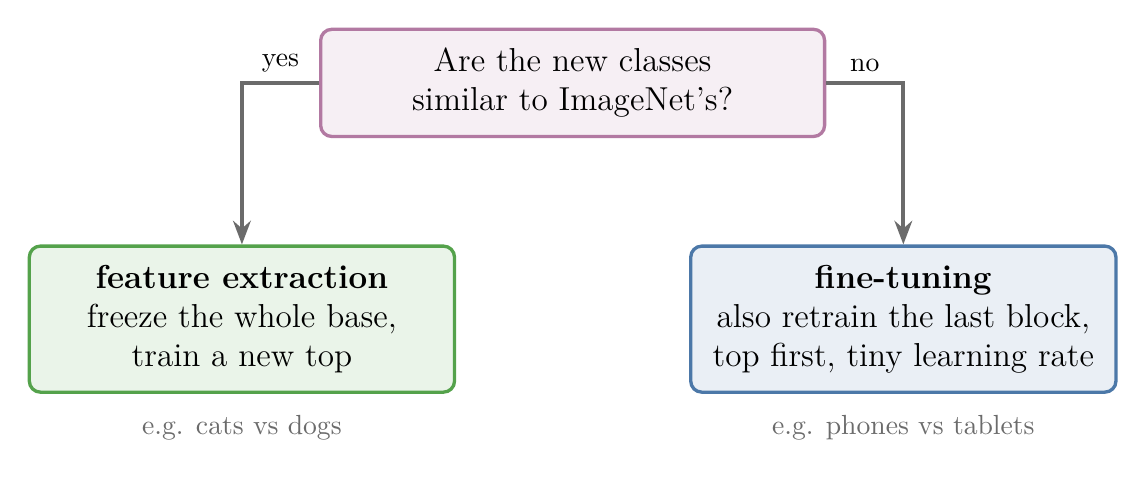
\begin{tikzpicture}[lab/.style={font=\sffamily\normalsize, align=center}]
  \node[box=cpurple, font=\sffamily\large, minimum width=6.4cm] (q) at (0,0) {Are the new classes\\similar to ImageNet's?};
  \node[box=cgreen, font=\sffamily\large, minimum width=5.4cm] (fe) at (-4.2,-3.0) {\textbf{feature extraction}\\freeze the whole base,\\train a new top};
  \node[box=cblue, font=\sffamily\large, minimum width=5.4cm] (ft) at (4.2,-3.0) {\textbf{fine-tuning}\\also retrain the last block,\\top first, tiny learning rate};
  \draw[arrow] (q) -| node[lab, pos=0.25, above] {yes} (fe);
  \draw[arrow] (q) -| node[lab, pos=0.25, above] {no} (ft);
  \node[lab, text=cgrey, below=4pt of fe] {e.g. cats vs dogs};
  \node[lab, text=cgrey, below=4pt of ft] {e.g. phones vs tablets};
\end{tikzpicture}
\end{document}
